\begin{center}
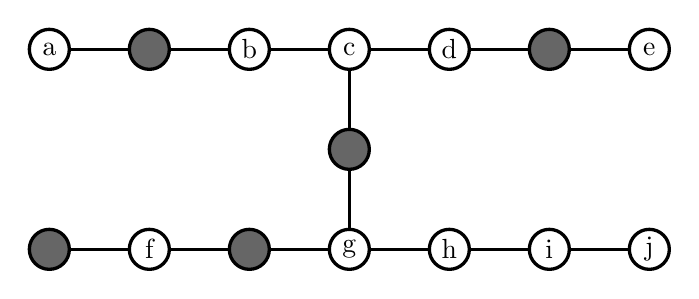
\begin{tikzpicture}[x=0.25in,y=0.25in]
  \draw [very thick]  (-6,2) -- (-4,2) -- (-2,2) -- (0,2) -- (2,2) -- (4,2) -- (6,2);
  \draw [very thick]  (-6,-2) -- (-4,-2) -- (-2,-2) -- (0,-2) -- (2,-2) -- (4,-2) -- (6,-2);
  \draw [very thick] (0,2) -- (0,-2);
    
    \draw [color = black, fill = white, very thick] (-6,2) circle (0.4);
      \node at (-6,2) {a};
    \draw [color = black, fill = black!60, very thick] (-4,2) circle (0.4);
    \draw [color = black, fill = white, very thick] (-2,2) circle (0.4);
      \node at (-2,2) {b};
    \draw [color = black, fill = white, very thick] (0,2) circle (0.4);
      \node at (0,2) {c};
    \draw [color = black, fill = white, very thick] (2,2) circle (0.4);
      \node at (2,2) {d};
    \draw [color = black, fill = black!60, very thick] (4,2) circle (0.4);
    \draw [color = black, fill = white, very thick] (6,2) circle (0.4);
      \node at (6,2) {e};

    \draw [color = black, fill = black!60, very thick] (-6,-2) circle (0.4);
    \draw [color = black, fill = white, very thick] (-4,-2) circle (0.4);
      \node at (-4,-2) {f};
    \draw [color = black, fill = black!60, very thick] (-2,-2) circle (0.4);
    \draw [color = black, fill = white, very thick] (0,-2) circle (0.4);
      \node at (0,-2) {g};
    \draw [color = black, fill = white, very thick] (2,-2) circle (0.4);
      \node at (2,-2) {h};
    \draw [color = black, fill = white, very thick] (4,-2) circle (0.4);
      \node at (4,-2) {i};
    \draw [color = black, fill = white, very thick] (6,-2) circle (0.4);
      \node at (6,-2) {j};

    \draw [color = black, fill = black!60, very thick] (0,0) circle (0.4);
  \end{tikzpicture}

\vfill

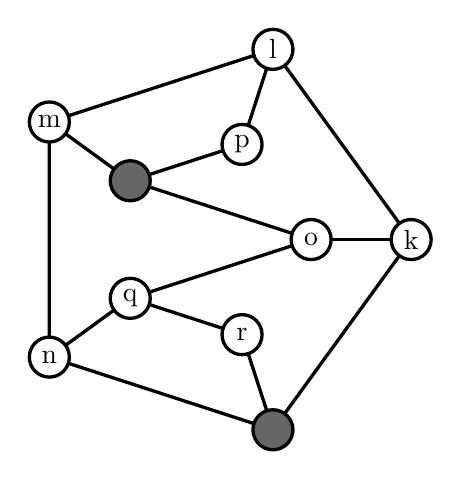
\begin{tikzpicture}[x=0.25in,y=0.25in]
    \draw [very thick] (0:4) -- (0:2);
    \draw [very thick] (72:4) -- (72:2);
    \draw [very thick] (144:4) -- (144:2);
    \draw [very thick] (-144:4) -- (-144:2);
    \draw [very thick] (-72:4) -- (-72:2);
    \draw [very thick] (0:4) -- (72:4) -- (144:4) -- (-144:4) -- (-72:4) -- (0:4);
    \draw [very thick] (72:2) -- (144:2) -- (0:2) -- (-144:2) -- (-72:2);

    \draw [color = black, fill = white, very thick] (0:4) circle (0.4);
      \node at (0:4) {k};
    \draw [color = black, fill = white, very thick] (72:4) circle (0.4);
      \node at (72:4) {l};
    \draw [color = black, fill = white, very thick] (144:4) circle (0.4);
      \node at (144:4) {m};
    \draw [color = black, fill = white, very thick] (-144:4) circle (0.4);
      \node at (-144:4) {n};
    \draw [color = black, fill = black!60, very thick] (-72:4) circle (0.4);
    \draw [color = black, fill = white, very thick] (0:2) circle (0.4);
      \node at (0:2) {o};
    \draw [color = black, fill = white, very thick] (72:2) circle (0.4);
      \node at (72:2) {p};
    \draw [color = black, fill = black!60, very thick] (144:2) circle (0.4);
    \draw [color = black, fill = white, very thick] (-144:2) circle (0.4);
      \node at (-144:2) {q};
    \draw [color = black, fill = white, very thick] (-72:2) circle (0.4);
      \node at (-72:2) {r};
  \end{tikzpicture}

\vfill

%\begin{tikzpicture}[x=0.25in,y=0.25in]
%    \draw [very thick] (-11,0) -- (-9,0) -- (-7,0) -- (-5,0) -- (-3,0) -- (-2,2) -- (0,3) -- (2,2) -- (3,0) -- (2,-2) -- (0,-3) -- (-2,-2) -- (-3,0);
%    
%    \draw [color = black, fill = white, very thick] (-11,0) circle (0.4);
%    \draw [color = black, fill = white, very thick] (-9,0) circle (0.4);
%    \draw [color = black, fill = white, very thick] (-7,0) circle (0.4);
%    \draw [color = black, fill = white, very thick] (-5,0) circle (0.4);
%    \draw [color = black, fill = white, very thick] (-3,0) circle (0.4);
%    \draw [color = black, fill = white, very thick] (3,0) circle (0.4);
%    \draw [color = black, fill = white, very thick] (0,-3) circle (0.4);
%    \draw [color = black, fill = white, very thick] (0,3) circle (0.4);
%    \draw [color = black, fill = white, very thick] (2,2) circle (0.4);
%    \draw [color = black, fill = white, very thick] (-2,2) circle (0.4);
%    \draw [color = black, fill = white, very thick] (2,-2) circle (0.4);
%    \draw [color = black, fill = white, very thick] (-2,-2) circle (0.4);
%  \end{tikzpicture}
%
%\vfill

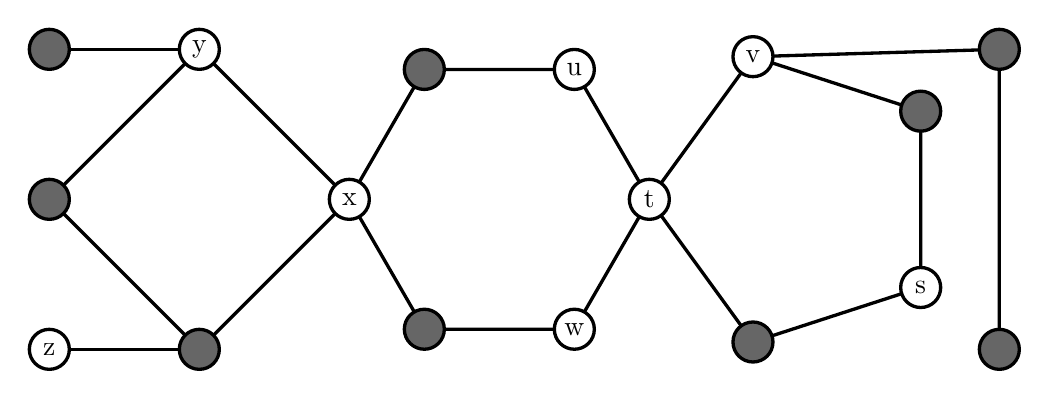
\begin{tikzpicture}[x=0.25in,y=0.25in]
\begin{scope}[shift={(0:3)}]   
    \draw [very thick] (-180:3) -- (-108:3) -- (-36:3) -- (36:3) -- (108:3) -- cycle;
    \draw [very thick] (108:3) -- (4,3) -- (4,-3);
%    \draw [color = black, fill = white, very thick] (-180:3) circle (0.4);
    \draw [color = black, fill = black!60, very thick] (-108:3) circle (0.4);
    \draw [color = black, fill = black!60, very thick] (36:3) circle (0.4);
    \draw [color = black, fill = white, very thick] (-36:3) circle (0.4);
      \node at (-36:3) {s};
    \draw [color = black, fill = white, very thick] (108:3) circle (0.4);
      \node at (108:3) {v};
    \draw [color = black, fill = black!60, very thick] (4,3) circle (0.4);
    \draw [color = black, fill = black!60, very thick] (4,-3) circle (0.4);
\end{scope}
\begin{scope}[shift={(0:-3)}] 
    \draw [very thick] (-180:3) -- (-120:3) -- (-60:3) -- (0:3) -- (60:3) -- (120:3) -- cycle;
    \draw [color = black, fill = white, very thick] (0:3) circle (0.4);
      \node at (0:3) {t};
    \draw [color = black, fill = white, very thick] (60:3) circle (0.4);
      \node at (60:3) {u};
    \draw [color = black, fill = black!60, very thick] (120:3) circle (0.4);
%    \draw [color = black, fill = white, very thick] (180:3) circle (0.4);
    \draw [color = black, fill = black!60, very thick] (-120:3) circle (0.4);
    \draw [color = black, fill = white, very thick] (-60:3) circle (0.4);
      \node at (-60:3) {w};
\end{scope}
\begin{scope}[shift={(0:-9)}] 
    \draw [very thick] (-180:3) -- (-90:3) -- (0:3) -- (90:3) -- cycle;
    \draw [very thick] (0,-3) -- (-3,-3);
    \draw [very thick] (0,3) -- (-3,3);
    \draw [color = black, fill = white, very thick] (0:3) circle (0.4);
      \node at (0:3) {x};
    \draw [color = black, fill = white, very thick] (90:3) circle (0.4);
      \node at (90:3) {y};
    \draw [color = black, fill = black!60, very thick] (180:3) circle (0.4);
    \draw [color = black, fill = black!60, very thick] (-90:3) circle (0.4);
    \draw [color = black, fill = white, very thick] (-3,-3) circle (0.4);
      \node at (-3,-3) {z};
    \draw [color = black, fill = black!60, very thick] (-3,3) circle (0.4);
\end{scope}
  \end{tikzpicture}
  \end{center}

\vfill

\begin{center}TOTAL BUDGET: \$12000\end{center}
